\let\negmedspace\undefined
\let\negthickspace\undefined
\documentclass[journal,12pt,twocolumn]{IEEEtran}
\usepackage{cite}
\usepackage{amsmath,amssymb,amsfonts,amsthm}
\usepackage{algorithmic}
\usepackage{graphicx}
\usepackage{textcomp}
\usepackage{xcolor}
\usepackage{txfonts}
\usepackage{listings}
\usepackage{enumitem}
\usepackage{mathtools}
\usepackage{gensymb}
\usepackage{comment}
\usepackage[breaklinks=true]{hyperref}
\usepackage{tkz-euclide} 
\usepackage{listings}
\usepackage{gvv}                                        
\def\inputGnumericTable{}                                 
\usepackage[latin1]{inputenc}                                
\usepackage{color}                                            
\usepackage{array}                                            
\usepackage{longtable}                                       
\usepackage{calc}                                             
\usepackage{multirow}                                         
\usepackage{hhline}                                           
\usepackage{ifthen}                                           
\usepackage{lscape}

\newtheorem{theorem}{Theorem}[section]
\newtheorem{problem}{Problem}
\newtheorem{proposition}{Proposition}[section]
\newtheorem{lemma}{Lemma}[section]
\newtheorem{corollary}[theorem]{Corollary}
\newtheorem{example}{Example}[section]
\newtheorem{definition}[problem]{Definition}
\newcommand{\BEQA}{\begin{eqnarray}}
\newcommand{\EEQA}{\end{eqnarray}}
\newcommand{\define}{\stackrel{\triangle}{=}}
\theoremstyle{remark}
\newtheorem{rem}{Remark}

\usepackage{graphicx}
\graphicspath{ {./Downloads/} }
\begin{document}

\bibliographystyle{IEEEtran}
\vspace{3cm}

\title{GATE 2021}
\author{EE22BTECH11060 - TEJAVATH KUSHAL$^{*}$% <-this % stops a space
}
\maketitle
\newpage
\bigskip

\renewcommand{\thefigure}{\theenumi}
\renewcommand{\thetable}{\theenumi}


\maketitle
\noindent \textbf{Q.40} : 
For a unit step input \( u[n] \), a discrete-time LTI system produces an output signal \( (2\delta[n+1]+\delta[n]+\delta[n-1]) \). Let \( y[n] \) be the output of the system for an input \( \brak{\brak{\frac{1}{2}^n}u[n]} \). The value of \( y[0] \) is:
\begin{flushright}
\brak{\text{GATE 2021 EC}}
\end{flushright}

\noindent \textbf{Ans.}

\begin{table}[h]
  \centering
\begin{tabular}{|c|c|}
        \hline
        \textbf{Input} & \textbf{Output} \\
        \hline
        $u[n]$ & $2\delta[n+1]+\delta[n]+\delta[n-1]$ \\ 
	\hline
	$\brak{\frac{1}{2}}^nu[n]$ & $y[n]$  \\ 
        \hline
\end{tabular}
\caption{Input-Output parameter table}
\label{tab:gate.2023.ec.40.1}





\end{table}

\noindent For impulse response
\begin{align}
h\brak{n}&=s\brak{n}-s\brak{n-1}\\
\notag h\brak{n} &=2\delta\brak{n+1}+\delta\brak{n}+\delta\brak{n-1}-2\delta\brak{n} \\
&~~~~~~~~~~~~~~-\delta\brak{n-1}-\delta\brak{n-1-1}\\
\implies h\brak{n} &=2\delta\brak{n+1}-\delta\brak{n}-\delta\brak{n-2}
\end{align}
\text{For input }$x\brak{n}=\brak{\frac{1}{2}}^nu\brak{n}$
\begin{align}
y\brak{n} &= x\brak{n}*h\brak{n}\\
 &= x\brak{n}*[2\delta\brak{n+1}-\delta\brak{n}-\delta\brak{n-2}]\\
 &= 2x\brak{n+1}-x\brak{n}-x\brak{n-2}\\
\notag  &=2\brak{\frac{1}{2}}^{n+1}u\brak{n+1}-\brak{\frac{1}{2}}^nu\brak{n}\\
&~~~~~~~~~~~~~~~~~~~-\brak{\frac{1}{2}}^{n-2}u\brak{n-2}\\
\notag y\brak{0} &=2\brak{\frac{1}{2}}^{0+1}u\brak{0+1}-\brak{\frac{1}{2}}^0u\brak{0}\\
&~~~~~~~~~~~~~~~~~~~-\brak{\frac{1}{2}}^{0-2}u\brak{0-2}\\
\implies y\brak{0} &=0
\end{align}\\
\pagebreak
\begin{figure}[h]
    %\caption{ Plot of $y\brak{n}$ v/s n}
    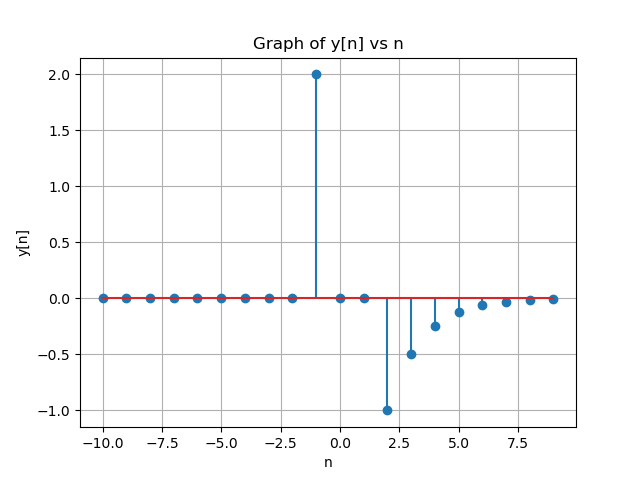
\includegraphics[width=0.5\textwidth]{figs/y(n) vs n.png}\label{fig:stem plot}
    \caption{Plot of $y\brak{n}$ v/s n}
\end{figure}




\end{document}
